%-----------------------------------------------------------------------------------------------------
% MAIN PROGRAM OF THESIS
%-----------------------------------------------------------------------------------------------------

% Set the class of document for NYCU-Thesis
% Availbale Class:
%   模式：[draft] | final （初稿 | 定稿）
%        draft - 會幫你在封面加上"初稿"
%        final - 就是正式版的東西，nothing special
%                不管哪一個都會有校徽浮水印，因為我不喜歡"DRAFT"浮水印，很醜
%   用途：[print] | upload （輸出 | 上傳）
%        print - 輸出是指印出來的時候會包含的東西，所以會幫你把那一堆審定書、授權書都加上來。
%        upload - 是拿來上傳圖書館用的，就不會有那一堆文件。
\documentclass[draft, print]{Class/NYCU-Thesis}

%-----------------------------------------------------------------------------------------------------
% 參數設定們
%-----------------------------------------------------------------------------------------------------

% 請去Config/config.tex填一些關於這本論文的參數
%----------------------------------------------------------------------
% 參數設定
% 這邊就是一些等一下模板在生出像是封面這些東西的時候，會需要用到的參數
%----------------------------------------------------------------------

% 中英文論文題目
\zhTitle{基於一致性方法之多詞元預測研究：選擇性分布一致性與潛在一致性匹配}
\enTitle{Multi-Token Prediction with Consistency Methods: Selective Distribution Consistency + Latent Consistency Matching}

% 中英文關鍵字
%       - 依據學校規定
%           關鍵詞 5-7 個，應附於摘要內
\zhKeywords{多詞元預測、一致性學習、選擇性分布一致性、潛在一致性匹配、大型語言模型}
\enKeywords{Multi-Token Prediction, Consistency Learning, Selective Distribution Consistency, Latent Consistency Matching, Large Language Models}

% 研究生中英文姓名
%       - 依據學校提供的範例
%           英文姓名應寫「姓, 名」，例：Wang, Jing
\zhStudentName{陳九龍}
\enStudentFirstName{Chen}
\enStudentLastName{Jiou-Lung}

% 指導教授中英文姓名
%       - 依據學校提供的範例
%           英文姓名應寫「姓, 名」，例：Wang, Jing
\zhAdvisorName{馬清文}
\enAdvisorFirstName{MA}
\enAdvisorLastName{Ching-Wen}

% 中英文學校名稱
\zhUnivName{國立陽明交通大學}
\enUnivName{National Yang Ming Chiao Tung University}

% 中英文學院名稱
\zhCollegeName{智慧科學暨綠能學院}
\enCollegeName{College of Artificial Intelligence}

% 中英文研究所名稱
\zhInstName{智慧計算與科技研究所智慧物聯網產業碩士專班}
\enInstName{Institute of Intelligent Computing and Technology}

% 英文學位名稱
%       - 書名頁要用的
\enDegree{Master of Science}

% 英文領域名稱
%       - 書名頁要用的
%           出現在最下面的那一坨英文的最後一段文字
%       - 學校公版和系上的範本都有提供這個欄位
%           但是資科工所上傳審查的時候又說不用
%           所以如果不需要的話，可以留空就不會印東西出來。
\enField{Computer Science}

% 英文地點名稱
%       - 書名頁要用的
%           依據學校提供的範例，Taiwan, Republic of China
\enLocation{Taiwan, Republic of China}

% 論文中英文日期
\zhDegreeYear{一一五}
\zhDegreeMonth{八}
\enDegreeYear{2026}
\enDegreeMonth{August}

% Watermark of thesis (論文浮水印)
\watermark{Figures/watermark.png}
% 請去Config/fonts.tex填一下要用的字體
\input{Config/fonts}

%-----------------------------------------------------------------------------------------------------
% 開始寫內容啦
%-----------------------------------------------------------------------------------------------------

% 這個模板用的Bibliography管理器是biblatex
% biblatex規定要在\begin{document}前加入bib資料
\addbibresource{6-Reference/thesis.bib}

\begin{document}

% 以下註解的數字編號是參考自
% https://aa.nycu.edu.tw/reg/regulation/ 
% 底下的 博碩士學位論文格式規範(中、英文說明)。
% 窩有留一份在Others裡面
% 最近一次更新是Sep. 16th, 2023

% 1. 封面頁
\makeCoverPage

% 2. 書名頁
\makeTitlePage

% 3. 論文電子檔著作權授權書
%       - 這邊提供的是學校的公版文件：
%           https://aa.nycu.edu.tw/reg/regulation/
%       - 口試完將修改完的論文檔案上傳到：
%           https://etd.lib.nctu.edu.tw/cgi-bin/gs32/tugsweb.cgi?o=dwebmge
%           就會拿到填好的各種授權書，所以這是輸出且為定稿才會出現的東西。
%       - 如果有多份授權書需加入，如授權書與延後公開申請書，
%           請先合併成一個PDF然後在這邊指定路徑。
\makeAuthPage{1-Authorization/1-Authorization.pdf}

% 4. 博士論文指導教授推薦書(碩士論文免附)
%       - 窩只有碩士畢業，所以窩沒有這個東西R。
%           如果有需要，可以使用\includepdf來引入PDF檔案。

% 5. 論文審定同意書
%       - 這邊有附一個學校提供的公版：
%           https://aa.nycu.edu.tw/reg/regulation/
%           但假如是資訊學院的同學，可以直接在申請口試完後從系統匯出已經填好資料的這張表。
%       - 這一頁將不會出現在上傳版本中（學校的電子論文不需要這一張），
%           因此只會出現在列印輸出版中。
%           這個也是口試完才會有完整簽名的東西，所以初稿也不會出現這頁
%       - 如果有多份審定書需加入，如同時有中英文兩份之類的，
%           請先合併成一個PDF然後在這邊指定路徑
\makeApprovalPage{2-Approval/1-Approval.pdf}

% 6. 誌謝
%       依據學校的規定，可依個人意願自行決定是否撰寫，以不超過一頁為原則。
%       如果不想寫，就請將這一行註解。
%----------------------------------------------------------------------
% ACKNOWLEDGEMENT (誌謝)
%----------------------------------------------------------------------

\begin{acknowledgement}

    首先，感謝馬老師在研究期間給予我的指導與支持，讓我有機會投入大型語言模型預訓練相關研究。這類研究需要相當多的運算資源，若沒有老師提供的研究環境與資源支持，這份研究很難順利完成。

    也感謝家人在這段時間給我的支持與鼓勵，讓我能夠專心完成研究與論文。

    最後，感謝實驗室的同學們願意花時間和我討論研究內容，並在研究過程中提供許多建議與幫助，讓我在遇到問題時能有不同的想法與方向。

\end{acknowledgement}


% 請不要動這一行
% 這一行代表開始編頁碼，從這一行以後開始的頁面會編羅馬數字（i, ii, iii, ...）
% 依據學校的規定，中文摘要至圖表目錄等，以 i, ii, iii...等小寫羅馬數字連續編頁。
\frontmatter

% 7. 中文摘要
%----------------------------------------------------------------------
% 中文摘要
%----------------------------------------------------------------------

% 把中文摘要寫在裡面
\begin{zhAbstract}

    自回歸大型語言模型在推論過程中通常逐一生成詞元，使生成延遲隨輸出序列長度增加。多詞元預測（Multi-Token Prediction, MTP）透過共享模型主幹與多個預測頭，使模型能在單次前向傳播中同時預測多個未來詞元，因而具備加速解碼的潛力。然而，標準 MTP 主要由各預測頭針對其對應的真實詞元獨立計算交叉熵損失，缺乏不同預測頭之間的一致性約束，使距離當前位置較遠的未來詞元預測面臨較高的最佳化難度。

    為改善上述問題，本研究提出選擇性分布一致性（Selective Distribution Consistency, SDC），並結合潛在一致性匹配（Latent Consistency Matching, LCM），在不改變 MTP 模型架構的前提下，分別於輸出機率分布與潛在表示層級強化第一預測頭與其餘預測頭之間的一致性。SDC 以第一預測頭作為教師，利用其預測機率分布監督其餘學生預測頭，並透過信心度門檻排除低信心度位置，以降低不可靠教師訊號對一致性學習的影響；LCM 則透過均方誤差縮小教師與學生預測頭之隱藏表示差距。

    本研究以 OpenWebText 進行模型訓練，並透過各預測頭之 Oracle perplexity、平均可接受草稿詞元數（Average Draft Tokens Accepted）、生成文本 perplexity、entropy、4-gram repetition，以及跨資料集零樣本評估，分析所提方法對預測品質、草稿詞元接受能力與生成品質的影響。

    正式 1.3B 模型實驗結果顯示，相較於標準 MTP baseline，SDC 與 LCM 聯合訓練可降低四個預測頭的 perplexity，其中第四預測頭的降幅最大，達 5.9\%；平均可接受草稿詞元數提升 4.2\%；生成文本 perplexity 則降低 52.7\%。此外，跨資料集零樣本評估亦顯示，所提方法在多數資料集與預測頭上具有改善效果。整體而言，實驗結果顯示，透過輸出分布與潛在表示兩個層級的一致性學習，可改善較遠未來詞元預測頭的最佳化表現，並提升 MTP 的多詞元預測品質與草稿詞元接受能力，展現進一步提升解碼效率的潛力。

    % 這個Command會自動幫你把Config裡面設定的東東填進來
    \zhAbsKeywords
\end{zhAbstract}


% 8. 英文摘要
%----------------------------------------------------------------------
% 英文摘要
%----------------------------------------------------------------------

% 把英文摘要寫在裡面
\begin{enAbstract}

    Autoregressive large language models typically generate tokens sequentially during inference, causing generation latency to increase with the length of the output sequence. Multi-Token Prediction (MTP) enables a model to predict multiple future tokens within a single forward pass through a shared model trunk and multiple prediction heads, thereby providing the potential to accelerate decoding. However, standard MTP mainly trains each prediction head independently using the cross-entropy loss associated with its corresponding ground-truth token, without explicitly enforcing consistency across prediction heads. As a result, prediction heads responsible for tokens farther into the future are generally more difficult to optimize.

    To address this issue, this study proposes Selective Distribution Consistency (SDC) and combines it with Latent Consistency Matching (LCM). Without modifying the underlying MTP architecture, the proposed approach improves consistency between the first prediction head and the remaining prediction heads at both the output probability distribution and latent representation levels. SDC treats the first prediction head as the teacher and uses its predictive probability distribution to supervise the remaining student heads. A confidence threshold is further applied to exclude low-confidence positions, thereby reducing the influence of unreliable teacher signals during consistency learning. In contrast, LCM minimizes the discrepancy between the hidden representations of the teacher and student heads using the mean squared error.

    The models are trained on OpenWebText and evaluated using Oracle perplexity (Oracle PPL) for individual prediction heads, Average Draft Tokens Accepted, generative perplexity (Generative PPL), entropy, 4-gram repetition, and cross-dataset zero-shot evaluation. These metrics are used to assess the effects of the proposed methods on prediction quality, draft-token acceptance, and generation quality.

    Experimental results on the main 1.3B-parameter model show that, compared with the standard MTP baseline, joint training with SDC and LCM reduces perplexity across all four prediction heads, with the largest improvement of 5.9\% observed for the fourth prediction head. The Average Draft Tokens Accepted increases by 4.2\%, while Generative PPL decreases by 52.7\%. Cross-dataset zero-shot evaluation further demonstrates improvements across most datasets and prediction heads. Overall, the results indicate that enforcing consistency at both the output distribution and latent representation levels improves the optimization of prediction heads responsible for more distant future tokens, increases draft-token acceptance, and demonstrates the potential for more efficient MTP decoding.

    % 這個Command會自動幫你把Config裡面設定的東東填進來    
    \enAbsKeywords
\end{enAbstract}


% 9. 目錄
\maketoc

% 10. 圖目錄
%       - 如果沒有可以註解掉
\makelof

% 11. 表目錄
%       - 如果沒有可以註解掉
\makelot

% 請不要動這一行
% 這一行代表開始編頁碼，從這一行以後開始的頁面會編阿拉伯數字（1, 2, 3, ...）
% 依據學校的規定，論文第一章以至附錄，均以 1，2，3…等阿拉伯數字連續編頁。
\mainmatter

% 12. 論文正文
%       - 各章節內容，窩有在裡面附一些常用的Sample。
%           如果有需要，可隨意增減檔案。
%----------------------------------------------------------------------
% 緒論
%----------------------------------------------------------------------

\chapter{Introduction}\label{chap:intro}

In recent years, to mitigate the inference latency caused by token-by-token generation in autoregressive large language models, researchers have begun exploring approaches that predict multiple future tokens within a single model inference step. Gloeckle et al.\cite{gloeckle2024mtp} introduced Multi-Token Prediction (MTP), which enables the model to simultaneously predict tokens at multiple future positions during pre-training through a shared model trunk and multiple prediction heads. Subsequently, Samragh et al.\cite{samragh2025future} further investigated how multi-token prediction capabilities can be introduced into existing pretrained language models through supervised fine-tuning and additional consistency objectives. In addition, DeepSeek-V3\cite{deepseekai2024deepseekv3} incorporated MTP into the pre-training objective of a large-scale language model, demonstrating the practical potential of multi-token prediction for improving inference efficiency.

\section{Background and Motivation}\label{sec:1-motivation}

\subsection{Background}

Large language models typically generate text in an autoregressive manner. Given an input sequence, the model predicts the next token based on the previously observed tokens, appends the newly generated token to the sequence, and then performs the next prediction step. Although this next-token prediction paradigm preserves a clear causal dependency, inference generally requires tokens to be generated sequentially. As a result, the number of forward passes increases with the length of the output sequence.

Multi-Token Prediction (MTP) extends conventional next-token prediction to multiple future positions. An MTP model consists of a shared model trunk and multiple prediction heads. Given the same input representation, the first prediction head predicts the next token, while the remaining prediction heads are responsible for predicting tokens at more distant future positions. Consequently, multiple future-token predictions can be obtained from a single forward pass through the shared model trunk. Since most of the computational cost is concentrated in the shared trunk, while the additional cost introduced by multiple prediction heads is relatively limited, MTP provides the potential to reduce redundant model computation and accelerate decoding.

During inference, the future tokens generated by multiple prediction heads can be treated as draft tokens. If these draft tokens are consistent with the subsequent verification results, multiple tokens can be accepted within a single decoding step, thereby reducing the number of model forward passes required by conventional token-by-token generation. Therefore, the accuracy of future-token prediction and the reliability of the outputs produced by different prediction heads directly affect the potential decoding efficiency of MTP.

\subsection{Motivation}

Although Multi-Token Prediction (MTP) provides a promising approach for accelerating autoregressive decoding, effectively optimizing multiple prediction heads remains challenging. In standard MTP training, each prediction head is independently optimized using the cross-entropy loss associated with its corresponding ground-truth token. While this objective allows each head to learn future-token prediction, it does not explicitly enforce consistency among the predictions produced by different heads.

As the prediction horizon increases, the uncertainty of future-token prediction also increases. Consequently, prediction heads responsible for more distant future positions are generally more difficult to optimize and tend to exhibit lower prediction accuracy than the first prediction head. Since the effectiveness of multi-token decoding depends on the quality and reliability of the predicted draft tokens, inaccurate predictions from later heads may reduce the number of draft tokens that can be successfully accepted during decoding.

Based on these observations, this study investigates whether additional consistency constraints can improve the optimization of future-token prediction heads without modifying the underlying MTP architecture. Specifically, the first prediction head, which performs next-token prediction, is used as a relatively reliable reference to guide the remaining prediction heads. By encouraging consistency across prediction heads at both the output probability distribution and latent representation levels, this study aims to improve the prediction quality of distant future-token heads and enhance the effectiveness of multi-token decoding.

\section{Contributions}\label{sec:1-contribution}

\begin{enumerate}
    \item We propose Selective Distribution Consistency for MTP training, which aligns the output distributions of student heads with the first prediction head while filtering low-confidence teacher predictions.

    \item We combine SDC with Latent Consistency Matching (LCM) to improve consistency across prediction heads at both the output distribution and latent representation levels without modifying the MTP architecture.

    \item Experiments on a 1.3B-parameter model show that SDC+LCM reduces Oracle PPL across prediction heads, increases Average Draft Tokens Accepted, and substantially reduces Generative PPL.

\end{enumerate}


% \section{章節概述\small{（列點的方式）}}

% \begin{itemize}
%     \item 在這種困難的抉擇下，本人思來想去，寢食難安。 要想清楚，章節概述，到底是一種怎麽樣的存在。 塞涅卡在不經意間這樣說過，生命如同寓言，其價值不在與長短，而在與內容。這啟發了我。
%     \item 那麽， 既然如此， 斯賓諾莎在不經意間這樣說過，最大的驕傲於最大的自卑都表示心靈的最軟弱無力。這不禁令我深思。
%     \item 要想清楚，章節概述，到底是一種怎麽樣的存在。 了解清楚章節概述到底是一種怎麽樣的存在，是解決一切問題的關鍵。
%     \item 就我個人來說，章節概述對我的意義，不能不說非常重大。 馮學峰曾經說過，當一個人用工作去迎接光明，光明很快就會來照耀著他。帶著這句話，我們還要更加慎重的審視這個問題。
% \end{itemize}
%----------------------------------------------------------------------
% 文獻討討
%----------------------------------------------------------------------

\chapter{Related Work}\label{chap:related_works}

\section{Multi-Token Prediction}\label{sec:2-mtp}

Multi-Token Prediction (MTP) extends conventional next-token prediction by enabling a language model to predict multiple future tokens simultaneously. Gloeckle et al.\cite{gloeckle2024mtp} proposed an MTP framework consisting of a shared model trunk and multiple prediction heads, where each head is responsible for predicting a different future token. Their results showed that MTP can improve model performance and support self-speculative decoding for faster inference.

Samragh et al.\cite{samragh2025future} further explored introducing multi-token prediction capabilities into pretrained autoregressive language models through supervised fine-tuning. Their method incorporates additional training objectives, including consistency learning, to improve the accuracy and coherence of jointly predicted future tokens while enabling faster decoding.

\section{Speculative Decoding}\label{sec:2-speculative_decoding}

Stern et al.\cite{stern2018blockwise} proposed Blockwise Parallel Decoding, an early approach for accelerating autoregressive generation by predicting multiple future tokens in parallel. The predicted tokens are then validated by a scoring model, and the longest valid prefix is accepted at each decoding step.

Leviathan et al.\cite{leviathan2023speculative} introduced speculative decoding, in which a lightweight draft model generates multiple candidate tokens that are subsequently verified in parallel by a larger target model. This approach reduces the number of sequential decoding steps while preserving the output distribution of the target model.

Cai et al.\cite{cai2024medusa} proposed Medusa, which eliminates the need for a separate draft model by adding multiple decoding heads to the target model. These heads predict multiple future tokens in parallel, while a tree-based attention mechanism is used to construct and verify candidate continuations efficiently.

\section{Consistency Learning}\label{sec:2-consistency_learning}

Consistency learning has been widely used as a regularization strategy to improve the stability and generalization of neural networks. Liang et al.\cite{liang2021rdrop} proposed R-Drop, which minimizes the bidirectional KL divergence between the output distributions of two sub-models generated by dropout, thereby encouraging consistent predictions under different stochastic perturbations.

Ni et al.\cite{ni2024lrdrop} extended consistency regularization from the output level to intermediate representations in Transformer-based language models. Their LR-Drop method aligns hidden states, attention matrices, and output distributions between different dropout-based sub-models, demonstrating that consistency constraints can be applied at multiple representation levels.

For multi-token prediction, Samragh et al.\cite{samragh2025future} introduced auxiliary consistency objectives to improve the coherence and accuracy of jointly predicted future tokens. Their approach applies consistency learning during supervised fine-tuning, showing that explicitly constraining future-token predictions can improve multi-token generation performance.

\section{Research Gap}\label{sec:2-research_gap}

Existing studies have demonstrated the potential of multi-token prediction for improving future-token prediction and accelerating autoregressive decoding. However, standard MTP primarily optimizes each prediction head independently using its corresponding ground-truth token, without explicitly leveraging the more reliable next-token prediction head to guide the optimization of later prediction heads. This issue becomes more significant as the prediction horizon increases, since predicting more distant future tokens is inherently more difficult.

Although previous studies \cite{samragh2025future} have introduced consistency-based objectives for multi-token prediction, the reliability of the teacher predictions used for consistency supervision has received relatively limited attention. In particular, directly enforcing consistency at low-confidence positions may introduce unreliable supervisory signals. Furthermore, consistency across both output probability distributions and latent representations has not been systematically investigated within the same MTP training framework. These limitations motivate the development of a selective consistency mechanism for improving the optimization of future-token prediction heads.
%----------------------------------------------------------------------
% 設計方法
%----------------------------------------------------------------------

\chapter{Proposed Method}\label{chap:method}

The proposed method introduces consistency objectives into the MTP training process while keeping the model architecture identical to the original MTP design. The overall training objective consists of the original MTP cross-entropy loss, Selective Distribution Consistency (SDC), and Latent Consistency Matching (LCM).

\section{MTP Training Objective}\label{sec:3-mtp_training_objective}

Given $K$ prediction heads, each head predicts a token at a different future position and is optimized using the cross-entropy loss with its corresponding ground-truth token. The baseline MTP objective is defined as

\begin{equation}
    \mathcal{L}_{\mathrm{MTP}}=\sum_{k=1}^{K}\mathcal{L}_{\mathrm{CE}}^{(k)},
\end{equation}

where $\mathcal{L}_{\mathrm{CE}}^{(k)}$ denotes the cross-entropy loss of the $k$-th prediction head for its corresponding future target token. This objective is retained as the primary token prediction loss in the proposed training framework.

\section{Selective Distribution Consistency}\label{sec:3-selective_distribution_consistency}

\begin{figure}[hpbt]
    \centering
    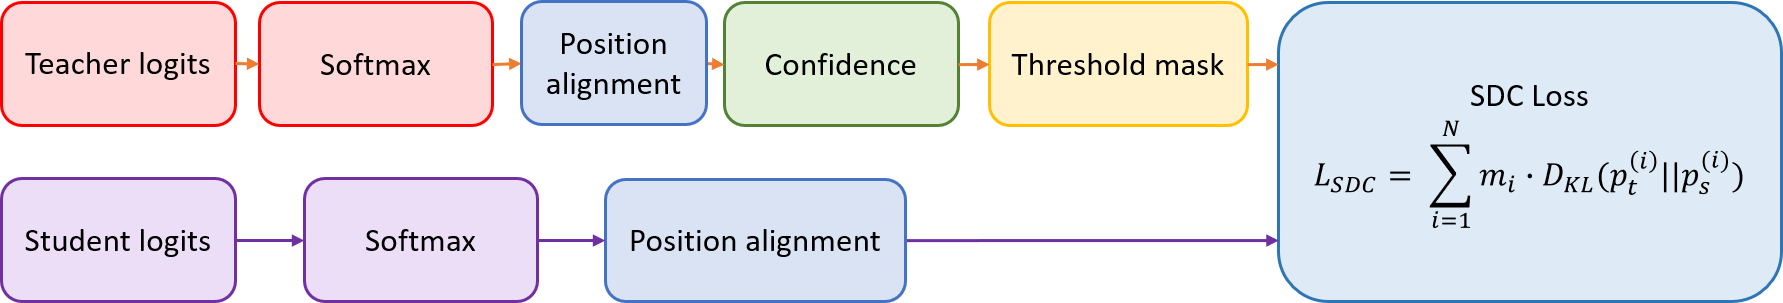
\includegraphics[width=\textwidth]{Figures/sdc_block_diagram.png}
    \caption{SDC block diagram.}
    \label{fig:sdc_block_diagram}
\end{figure}

Selective Distribution Consistency (SDC) aligns the output probability distributions of the student heads (Heads 2--$K$) with the teacher head (Head 1). Since different prediction heads correspond to different future offsets, the teacher and student predictions are first position-aligned such that they correspond to the same target token. Specifically, the prediction of Head $k$ at position $i$ is aligned with the prediction of Head 1 at position $i+k-1$.

For each token position, the teacher logits are first converted into a probability distribution using softmax:

\begin{equation}
    P_{t}^{(i)}=\operatorname{softmax}\left(z_{t}^{(i)}\right),
\end{equation}

where $P_{t}^{(i)}$ denotes the probability distribution produced by the teacher head (Head 1) at position $i$.

The confidence of the teacher prediction is then estimated using its normalized entropy:

\begin{equation}
    c_{i}=1-\frac{H\left(P_{t}^{(i)}\right)}{\log(V)},
\end{equation}

where $H(\cdot)$ denotes the entropy of the teacher probability distribution and $V$ is the vocabulary size. A higher $c_{i}$ indicates a more confident teacher prediction.

A confidence threshold $\tau$ is subsequently applied to construct a binary mask:

\begin{equation}
    m_{i}=\begin{cases}
                    1, & \text{if } c_{i} > \tau, \\
                    0, & \text{otherwise}.
                \end{cases}
\end{equation}

Thus, only token positions whose teacher confidence exceeds $\tau$ participate in consistency learning, while low-confidence positions are excluded from the SDC objective.

For the selected positions, the student probability distribution is encouraged to match the corresponding position-aligned teacher distribution by minimizing the KL divergence:

\begin{equation}
    \mathcal{L}_{\mathrm{SDC}}^{(k)}=\frac{1}{N_k}\sum_{i}m_{i+k-1}D_{\mathrm{KL}}\left(P_{t}^{(i+k-1)} \parallel P_{s}^{(i,k)}\right),
\end{equation}

where $P_{t}^{(i+k-1)}$ and $P_{s}^{(i,k)}$ denote the position-aligned teacher and student probability distributions corresponding to the same target token, respectively, and $N_k$ denotes the number of positions selected by the confidence mask for the $k$-th student head.

The overall SDC objective is defined as

\begin{equation}
    \mathcal{L}_{\mathrm{SDC}}=\sum_{k=2}^{K}\mathcal{L}_{\mathrm{SDC}}^{(k)}.
\end{equation}

This selective mechanism restricts distribution consistency learning to positions with sufficiently reliable teacher predictions.

\begin{algorithm}[htbp]
\caption{Selective Distribution Consistency}
\label{alg:sdc}

\KwIn{
Teacher logits $\{z_t^{(i)}\}$ from Head 1,
student logits $\{z_s^{(i,k)}\}_{k=2}^{K}$,
confidence threshold $\tau$
}

\KwOut{SDC loss $\mathcal{L}_{\mathrm{SDC}}$}

$\mathcal{L}_{\mathrm{SDC}} \leftarrow 0$\;

\ForEach{teacher position $i$}{
    $P_t^{(i)} \leftarrow \operatorname{softmax}\left(z_t^{(i)}\right)$\;
    
    $c_i \leftarrow
    1-\dfrac{H\left(P_t^{(i)}\right)}{\log V}$\;
    
    $m_i \leftarrow \mathbb{I}(c_i > \tau)$\;
}

\For{$k \leftarrow 2$ \KwTo $K$}{
    Align Head $k$ at position $i$ with Head 1 at position $i+k-1$\;
    
    $\mathcal{I}_k
    \leftarrow
    \{i \mid m_{i+k-1}=1\}$\;
    
    $N_k \leftarrow |\mathcal{I}_k|$\;
    
    $\mathcal{L}_{\mathrm{SDC}}^{(k)}
    \leftarrow
    \dfrac{1}{N_k}
    \displaystyle\sum_{i\in\mathcal{I}_k}
    D_{\mathrm{KL}}
    \left(
    P_t^{(i+k-1)}
    \parallel
    P_s^{(i,k)}
    \right)$\;
    
    $\mathcal{L}_{\mathrm{SDC}}
    \leftarrow
    \mathcal{L}_{\mathrm{SDC}}
    +
    \mathcal{L}_{\mathrm{SDC}}^{(k)}$\;
}

\Return{$\mathcal{L}_{\mathrm{SDC}}$}\;

\end{algorithm}

\section{Latent Consistency Matching}\label{sec:3-latent_consistency_matching}
Latent Consistency Matching (LCM) applies consistency learning at the latent representation level. The same position-alignment strategy used in SDC is applied to the hidden representations before latent consistency matching. Specifically, the hidden representation produced by the $k$-th student head is aligned with the representation produced by Head 1 that corresponds to the same target token.

For the $k$-th student head, the LCM loss is defined as

\begin{equation}
    \mathcal{L}_{\mathrm{LCM}}^{(k)}=\frac{1}{S_k D}\sum_{i=1}^{S_k}\sum_{d=1}^{D}\left(h_{t,i,d}^{(k)}-h_{s,i,d}^{(k)}\right)^2,
\end{equation}

where $h_{t,i,d}^{(k)}$ and $h_{s,i,d}^{(k)}$ denote the position-aligned teacher and student hidden representations, respectively, $S_k$ denotes the number of valid aligned token positions for the $k$-th student head, and $D$ denotes the hidden dimension.

The overall LCM objective is defined as

\begin{equation}
    \mathcal{L}_{\mathrm{LCM}}=\sum_{k=2}^{K}\mathcal{L}_{\mathrm{LCM}}^{(k)}.
\end{equation}

While SDC constrains the prediction heads at the output distribution level, LCM provides an additional consistency constraint on their position-aligned latent representations.
\section{Joint Training Objective}\label{sec:3-joint_training_objective}

The final training objective combines the original MTP loss with the two consistency objectives:

\begin{equation}\label{equ:joint_training_objective}
    \mathcal{L}_{\mathrm{total}} = \mathcal{L}_{\mathrm{MTP}} + \lambda_{\mathrm{SDC}}\mathcal{L}_{\mathrm{SDC}} + \lambda_{\mathrm{LCM}}\mathcal{L}_{\mathrm{LCM}},
\end{equation}

where $\lambda_{\mathrm{SDC}}$ and $\lambda_{\mathrm{LCM}}$ control the contributions of SDC and LCM, respectively.

During training, the teacher outputs are detached when computing the consistency objectives. Therefore, SDC and LCM use Head 1 as the reference to optimize Heads 2--$K$, while the original cross-entropy objective continues to optimize all prediction heads.

%----------------------------------------------------------------------
% 實驗設計分析
%----------------------------------------------------------------------

\chapter{Experimental Results}\label{chap:experimental_results}

\section{Experimental Setup and Evaluation Metrics}\label{sec:4-setup}

The main experiments were conducted using a 1.3B-parameter MTP model
with four prediction heads. The models were trained on
OpenWebText\cite{gokaslan2019openwebtext}. The baseline and proposed
models were trained on 10 billion tokens, while the ablation experiments
used models trained on 1 billion tokens. The main SDC+LCM configuration
used $\lambda_{\mathrm{SDC}}=1.0$, $\tau=0.3$, and
$\lambda_{\mathrm{LCM}}=0.5$. Detailed training configurations are
provided in Appendix \ref{app:experimental-config}.

The baseline model was optimized using the original MTP training objective,
whereas the proposed model additionally incorporated Selective Distribution
Consistency (SDC) and Latent Consistency Matching (LCM). Both settings used
the same MTP architecture, allowing the effects of the consistency objectives
to be evaluated independently of architectural changes.

Unless otherwise specified, values reported with $\pm$ denote the
mean $\pm$ standard deviation over three random seeds.

The models were evaluated in terms of prediction quality, draft-token
acceptance, generation quality, and cross-dataset generalization.
The corresponding evaluation procedures and results are described
in the following sections.

\section{Main Experimental Results}\label{sec:4-main_results}

\subsection{Oracle Perplexity}

Oracle PPL was computed independently for each prediction head using
its corresponding ground-truth future token, where lower PPL indicates
better prediction quality.

\begin{table}[!htbp]
    \centering
    \caption{Oracle PPL comparison between the baseline and SDC+LCM.}
    \label{tab:oracle_ppl}
    \begin{tabular}{lcccc}
        \toprule[1.25pt]
        Setting & Head 1 & Head 2 & Head 3 & Head 4 \\
        \midrule
        Baseline
        & 19.4293 & 87.2351 & 200.0813 & 318.3247 \\

        SDC+LCM
        & \textbf{19.1695}
        & \textbf{83.7266}
        & \textbf{189.2825}
        & \textbf{299.5625} \\

        Improvement
        & 1.34\%
        & 4.02\%
        & 5.40\%
        & \textbf{5.89\%} \\
        \bottomrule[1.25pt]
    \end{tabular}
\end{table}

Table \ref{tab:oracle_ppl} compares the Oracle PPL of the baseline MTP model and the proposed SDC+LCM model across four prediction heads. The proposed method consistently reduces PPL for all prediction heads. Head 1 shows a relatively small improvement of 1.34\%, whereas larger improvements are observed for the later prediction heads. Specifically, the PPL reductions for Heads 2, 3, and 4 are 4.02\%, 5.40\%, and 5.89\%, respectively.

The improvement becomes more pronounced as the prediction position moves farther into the future, with Head 4 achieving the largest reduction. This result indicates that consistency-based training is particularly beneficial for the optimization of later prediction heads, which are responsible for more distant future-token predictions. Although the consistency objectives primarily constrain Heads 2–4, a slight improvement is also observed for Head 1.

\subsection{Draft Token Acceptance}\label{subsec:draft_token_acceptance}

\begin{table}[!htbp]
    \centering
    \caption{Comparison of Average Draft Tokens Accepted between the baseline and SDC+LCM.}
    \label{tab:draft_token_acceptance}
    \begin{tabular}{lccccc}
        \toprule[1.25pt]
        Setting
        & Overall
        & Prefix 128
        & Prefix 256
        & Prefix 512
        & Prefix 768 \\
        \midrule

        Baseline
        & 0.7010
        & 0.9117 $\pm$ 0.0205
        & 0.9458 $\pm$ 0.0068
        & 0.9689 $\pm$ 0.0221
        & 0.9760 $\pm$ 0.0222 \\

        SDC+LCM
        & \textbf{0.7302}
        & \textbf{0.9653 $\pm$ 0.0401}
        & \textbf{0.9873 $\pm$ 0.0063}
        & \textbf{1.0158 $\pm$ 0.0309}
        & \textbf{1.0272 $\pm$ 0.0250} \\

        Improvement
        & 4.17\%
        & \textbf{5.88\%}
        & 4.39\%
        & 4.84\%
        & 5.25\% \\
        \bottomrule[1.25pt]
    \end{tabular}
\end{table}

Draft-token acceptance was evaluated using greedy predictions from the
MTP heads. Head 1 was used as the verification reference, while predictions
from Heads 2--$K$ were treated as draft tokens. Draft tokens were accepted
sequentially when they matched the corresponding Head 1 predictions, and
verification stopped at the first mismatch. Head 1 itself was not included
in the accepted draft-token count.

Average Draft Tokens Accepted denotes the average number of consecutively
accepted draft tokens per evaluation instance. The overall result was computed
over all valid positions, while additional evaluations were conducted using
random contiguous prefixes of lengths 128, 256, 512, and 768.

Table \ref{tab:draft_token_acceptance} compares the Average Draft Tokens
Accepted between the baseline and SDC+LCM. The proposed method increases
the overall Average Draft Tokens Accepted from 0.7010 to 0.7302,
corresponding to an improvement of 4.17\%.

Consistent improvements are also observed across different prefix lengths.
At prefix lengths of 128, 256, 512, and 768, SDC+LCM achieves improvements
of 5.88\%, 4.39\%, 4.84\%, and 5.25\%, respectively. Among these settings,
the largest improvement is observed at a prefix length of 128, while the
highest absolute number of accepted draft tokens is achieved at a prefix
length of 768.

These results indicate that the proposed consistency objectives improve
the reliability of future-token predictions, resulting in more draft tokens
being accepted under the self-speculative decoding criterion.

\subsection{Generative Quality}\label{subsec:generative_quality}

Generation quality was evaluated using Generative PPL, entropy, and
4-gram repetition. A total of 200 samples were generated using the first
128 tokens of each evaluation sequence as the prompt. Generation was
performed using top-$p$ and temperature sampling with $p=0.9$ and a
temperature of 0.8. Generative PPL was computed using GPT-2 Large as an
external language model, where only the generated continuation was included
in the perplexity calculation. Entropy was used to characterize the
diversity of generated tokens, while 4-gram repetition was used to measure
repetitive generation patterns.

\begin{table}[!htbp]
    \centering
    \caption{Comparison of generative quality between the baseline and SDC+LCM.}
    \label{tab:generative_quality}
    \begin{tabular}{lccc}
        \toprule[1.25pt]
        Setting
        & Generative PPL
        & Entropy
        & 4-gram Repetition \\
        \midrule

        Baseline
        & 39.5580 $\pm$ 0.9425
        & 7.3223 $\pm$ 0.0351
        & 0.0229 $\pm$ 0.0084 \\

        SDC+LCM
        & \textbf{18.7180 $\pm$ 0.8276}
        & 6.8620 $\pm$ 0.0202
        & 0.0526 $\pm$ 0.0147 \\

        Change
        & \textbf{-52.68\%}
        & -6.29\%
        & +130.17\% \\
        \bottomrule[1.25pt]
    \end{tabular}
\end{table}

Table \ref{tab:generative_quality} compares the generation quality of the
baseline and SDC+LCM models. The proposed method substantially reduces
Generative PPL from 39.5580 to 18.7180, corresponding to a reduction of
52.68\%. This result indicates that the generated text is evaluated as
more predictable by the external language model.

In addition, the entropy decreases from 7.3223 to 6.8620, representing
a reduction of 6.29\%. However, the 4-gram repetition increases from
0.0229 to 0.0526, corresponding to a relative increase of 130.17\%.

These results reveal a trade-off in generation behavior. Although
SDC+LCM significantly improves Generative PPL, the lower entropy and
higher 4-gram repetition indicate reduced generation diversity and an
increased tendency toward repetitive patterns. Nevertheless, the
absolute increase in 4-gram repetition is approximately 0.03.

\section{Zero-Shot Evaluation}\label{sec:zero_shot_evaluation}

\begin{table}[!htbp]
    \centering
    \caption{Zero-shot Oracle PPL improvement of SDC+LCM over the baseline across different datasets.}
    \label{tab:zero_shot_ppl}
    \begin{tabular}{lcccc}
        \toprule[1.25pt]
        Dataset
        & Head 1
        & Head 2
        & Head 3
        & Head 4 \\
        \midrule

        WikiText
        & 0.32\%
        & \textbf{7.57\%}
        & 7.19\%
        & 5.62\% \\

        PTB
        & \textbf{13.82\%}
        & 9.90\%
        & 10.53\%
        & 5.63\% \\

        LAMBADA
        & \textbf{38.53\%}
        & 10.43\%
        & 4.44\%
        & 3.27\% \\

        arXiv
        & 1.48\%
        & \textbf{3.94\%}
        & 3.71\%
        & 0.27\% \\

        PubMed
        & 7.04\%
        & 7.76\%
        & \textbf{8.33\%}
        & 8.26\% \\

        \bottomrule[1.25pt]
    \end{tabular}
\end{table}

To evaluate the generalization ability of the proposed method across
different domains, zero-shot evaluation was conducted on WikiText\cite{merity2016wikitext},
Penn Treebank (PTB)\cite{marcus1993ptb}, LAMBADA\cite{paperno2016lambada}, and the arXiv and PubMed subsets of the Scientific Papers dataset\cite{cohan2018scientificpapers}.
Table \ref{tab:zero_shot_ppl} reports the relative Oracle PPL improvement
of SDC+LCM over the baseline for each prediction head.

Overall, SDC+LCM achieves PPL improvements across all evaluated datasets
and prediction heads, although the magnitude of improvement varies
considerably across domains. For Head 1, relatively large improvements
are observed on PTB\cite{marcus1993ptb}, LAMBADA\cite{paperno2016lambada}, and PubMed\cite{cohan2018scientificpapers}, with LAMBADA\cite{paperno2016lambada} showing the
largest reduction of 38.53\%. In contrast, the improvement on WikiText\cite{merity2016wikitext}
is limited to 0.32\%.

For WikiText\cite{merity2016wikitext}, the improvements are mainly concentrated on Heads 2--4,
with reductions of 7.57\%, 7.19\%, and 5.62\%, respectively, while the
improvement for Head 1 is relatively limited.

The improvement patterns also vary for later prediction heads across
different domains. For example, Head 4 achieves an 8.26\% improvement
on PubMed but only a 0.27\% improvement on arXiv. These results indicate
that the effectiveness of consistency-based training depends partly on
the characteristics of the evaluation domain, while generally yielding improvements across unseen datasets.

\section{Ablation Study}\label{sec:ablation_study}

\subsection{Overall Ablation Results}\label{subsec:overall_ablation_results}

\begin{table}[!htbp]
    \centering
    \caption{Ablation results of Oracle PPL under different consistency settings.}
    \label{tab:ablation_oracle_ppl}
    \small
    \begin{tabular}{lcccc}
        \toprule[1.25pt]
        Setting
        & Head 1
        & Head 2
        & Head 3
        & Head 4 \\
        \midrule

        Baseline
        & 26.2356 
        & 121.8033 
        & 269.2450 
        & 406.6959  \\

        $\lambda_{SDC}=0.5,\ \tau=0.3,\ \lambda_{LCM}=0$
        & 26.4587 
        & 120.7186 
        & 265.0660 
        & 402.0413  \\
        
        $\lambda_{SDC}=1.5,\ \tau=0.3,\ \lambda_{LCM}=0$
        & 27.2684 
        & 122.5244 
        & 264.6119 
        & 397.3106  \\

        \midrule

        $\lambda_{SDC}=1.0,\ \tau=0.0,\ \lambda_{LCM}=0$
        & 26.7541 
        & 120.6687 
        & 261.6664 
        & 394.6503  \\

        $\lambda_{SDC}=1.0,\ \tau=0.3,\ \lambda_{LCM}=0$
        & 26.8150 
        & 120.5276 
        & 261.9479 
        & 394.7055  \\

        $\lambda_{SDC}=1.0,\ \tau=0.6,\ \lambda_{LCM}=0$
        & 27.7396 
        & 129.2922
        & 278.8881 
        & 417.5874  \\

        \midrule

        $\lambda_{SDC}=0,\ \tau=0,\ \lambda_{LCM}=0.5$
        & 25.7096 
        & 118.9247 
        & 262.1637 
        & 397.9911  \\

        $\lambda_{SDC}=0,\ \tau=0,\ \lambda_{LCM}=1.0$
        & 25.5312 
        & 118.5823 
        & 261.1872 
        & 395.1838  \\

        $\lambda_{SDC}=0,\ \tau=0,\ \lambda_{LCM}=1.5$
        & \textbf{25.4583} 
        & 119.1595 
        & 263.2083 
        & 398.8679  \\

        \midrule

        $\lambda_{SDC}=1.0,\ \tau=0.3,\ \lambda_{LCM}=0.5$
        & 26.2402 
        & \textbf{118.2168} 
        & 257.0344 
        & 387.7455  \\

        $\lambda_{SDC}=1.0,\ \tau=0.3,\ \lambda_{LCM}=1.0$
        & 26.4553 
        & 119.2975 
        & 258.4100 
        & 390.7829  \\

        $\lambda_{SDC}=1.5,\ \tau=0.3,\ \lambda_{LCM}=1.0$
        & 26.5485
        & 118.4341 
        & \textbf{254.9612} 
        & \textbf{383.7626}  \\

        \bottomrule[1.25pt]
    \end{tabular}

    \vspace{2mm}
    
    \footnotesize{\textit{Bold values indicate the best result in each column.}}
\end{table}

\begin{table}[!htbp]
    \centering
    \caption{Ablation results of Average Draft Tokens Accepted under different consistency settings.}
    \label{tab:ablation_draft_tokens}
    \resizebox{\textwidth}{!}{
        \begin{tabular}{lccccc}
            \toprule[1.25pt]
            Setting
            & Overall
            & Prefix 128
            & Prefix 256
            & Prefix 512
            & Prefix 768 \\
            \midrule

            Baseline
            & 0.6238
            & 0.8251 $\pm$ 0.0140
            & 0.8205 $\pm$ 0.0062
            & 0.8519 $\pm$ 0.0195
            & 0.8552 $\pm$ 0.0233 \\

            $\lambda_{SDC}=0.5,\ \tau=0.3,\ \lambda_{LCM}=0$
            & 0.6345
            & 0.8195 $\pm$ 0.0122
            & 0.8416 $\pm$ 0.0115
            & 0.8601 $\pm$ 0.0065
            & 0.8644 $\pm$ 0.0304 \\

            $\lambda_{SDC}=1.5,\ \tau=0.3,\ \lambda_{LCM}=0$
            & 0.6414
            & 0.8522 $\pm$ 0.0098
            & 0.8581 $\pm$ 0.0139
            & 0.8897 $\pm$ 0.0043
            & \textbf{0.9082 $\pm$ 0.0204} \\

            \midrule

            $\lambda_{SDC}=1.0,\ \tau=0.0,\ \lambda_{LCM}=0$
            & 0.6388
            & 0.8374 $\pm$ 0.0165
            & 0.8746 $\pm$ 0.0108
            & 0.8736 $\pm$ 0.0158
            & 0.8802 $\pm$ 0.0029 \\

            $\lambda_{SDC}=1.0,\ \tau=0.3,\ \lambda_{LCM}=0$
            & 0.6400
            & 0.8406 $\pm$ 0.0131
            & 0.8602 $\pm$ 0.0232
            & 0.8720 $\pm$ 0.0233
            & 0.8772 $\pm$ 0.0015 \\

            $\lambda_{SDC}=1.0,\ \tau=0.6,\ \lambda_{LCM}=0$
            & 0.6113
            & 0.7908 $\pm$ 0.0074
            & 0.7919 $\pm$ 0.0086
            & 0.8009 $\pm$ 0.0035
            & 0.8174 $\pm$ 0.0130 \\

            \midrule

            $\lambda_{SDC}=0,\ \tau=0,\ \lambda_{LCM}=0.5$
            & 0.6398
            & 0.8517 $\pm$ 0.0156
            & 0.8589 $\pm$ 0.0096
            & 0.8794 $\pm$ 0.0050
            & 0.8895 $\pm$ 0.0257 \\

            $\lambda_{SDC}=0,\ \tau=0,\ \lambda_{LCM}=1.0$
            & 0.6442
            & 0.8491 $\pm$ 0.0130
            & 0.8698 $\pm$ 0.0154
            & 0.8919 $\pm$ 0.0168
            & 0.8943 $\pm$ 0.0012 \\

            $\lambda_{SDC}=0,\ \tau=0,\ \lambda_{LCM}=1.5$
            & 0.6467
            & 0.8510 $\pm$ 0.0112
            & \textbf{0.8862 $\pm$ 0.0054}
            & 0.8951 $\pm$ 0.0129
            & 0.9028 $\pm$ 0.0327 \\

            \midrule

            $\lambda_{SDC}=1.0,\ \tau=0.3,\ \lambda_{LCM}=0.5$
            & 0.6507
            & 0.8498 $\pm$ 0.0339
            & 0.8615 $\pm$ 0.0179
            & 0.8987 $\pm$ 0.0103
            & 0.8862 $\pm$ 0.0151 \\

            $\lambda_{SDC}=1.0,\ \tau=0.3,\ \lambda_{LCM}=1.0$
            & 0.6495
            & 0.8402 $\pm$ 0.0209
            & 0.8612 $\pm$ 0.0043
            & 0.8879 $\pm$ 0.0157
            & 0.8950 $\pm$ 0.0071 \\

            $\lambda_{SDC}=1.5,\ \tau=0.3,\ \lambda_{LCM}=1.0$
            & \textbf{0.6525}
            & \textbf{0.8590 $\pm$ 0.0101}
            & 0.8656 $\pm$ 0.0214
            & \textbf{0.9023 $\pm$ 0.0277}
            & 0.9044 $\pm$ 0.0140 \\

            \bottomrule[1.25pt]
        \end{tabular}
    }
    \vspace{2mm}
    
    \footnotesize{\textit{Bold values indicate the best result in each column.}}
\end{table}

\begin{table}[!htbp]
    \centering
    \caption{Ablation results of generative quality under different consistency settings.}
    \label{tab:ablation_generation}
    \small
    \begin{tabular}{lccc}
        \toprule[1.25pt]
        Setting
        & Generative PPL
        & Entropy
        & 4-gram Repetition \\
        \midrule

        Baseline
        & 83.8285 $\pm$ 5.1409
        & 7.4068 $\pm$ 0.0461
        & 0.0119 $\pm$ 0.0097 \\

        $\lambda_{SDC}=0.5,\ \tau=0.3,\ \lambda_{LCM}=0$
        & 52.7654 $\pm$ 2.2732
        & 7.1490 $\pm$ 0.0335
        & 0.0323 $\pm$ 0.0169 \\

        $\lambda_{SDC}=1.5,\ \tau=0.3,\ \lambda_{LCM}=0$
        & 31.8082 $\pm$ 0.4503
        & 6.8248 $\pm$ 0.0353
        & 0.0485 $\pm$ 0.0159 \\

        \midrule

        $\lambda_{SDC}=1.0,\ \tau=0.0,\ \lambda_{LCM}=0$
        & 68.0596 $\pm$ 4.5760
        & 7.3141 $\pm$ 0.0519
        & 0.0193 $\pm$ 0.0154 \\

        $\lambda_{SDC}=1.0,\ \tau=0.3,\ \lambda_{LCM}=0$
        & 48.4875 $\pm$ 1.2280
        & 7.1184 $\pm$ 0.0336
        & 0.0183 $\pm$ 0.0055 \\

        $\lambda_{SDC}=1.0,\ \tau=0.6,\ \lambda_{LCM}=0$
        & 28.2332 $\pm$ 1.2754
        & 6.7789 $\pm$ 0.0178
        & 0.0393 $\pm$ 0.0080 \\

        \midrule

        $\lambda_{SDC}=0,\ \tau=0,\ \lambda_{LCM}=0.5$
        & 26.2091 $\pm$ 1.5675
        & 6.8576 $\pm$ 0.0374
        & 0.0555 $\pm$ 0.0204 \\

        $\lambda_{SDC}=0,\ \tau=0,\ \lambda_{LCM}=1.0$
        & 24.0955 $\pm$ 3.2440
        & 6.7935 $\pm$ 0.0828
        & 0.0657 $\pm$ 0.0388 \\

        $\lambda_{SDC}=0,\ \tau=0,\ \lambda_{LCM}=1.5$
        & 29.9033 $\pm$ 0.5373
        & 6.8644 $\pm$ 0.0249
        & 0.0215 $\pm$ 0.0049 \\

        \midrule

        $\lambda_{SDC}=1.0,\ \tau=0.3,\ \lambda_{LCM}=0.5$
        & \textbf{21.4788 $\pm$ 0.0773}
        & 6.6876 $\pm$ 0.0421
        & 0.0720 $\pm$ 0.0062 \\

        $\lambda_{SDC}=1.0,\ \tau=0.3,\ \lambda_{LCM}=1.0$
        & 26.3414 $\pm$ 0.3656
        & 6.7567 $\pm$ 0.0016
        & 0.0460 $\pm$ 0.0160 \\

        $\lambda_{SDC}=1.5,\ \tau=0.3,\ \lambda_{LCM}=1.0$
        & 25.7832 $\pm$ 1.6338
        & 6.7177 $\pm$ 0.0455
        & 0.0453 $\pm$ 0.0197 \\

        \bottomrule[1.25pt]
    \end{tabular}

    \vspace{2mm}
    
    \footnotesize{\textit{Bold indicates the lowest Generative PPL.}}
\end{table}

\FloatBarrier

\subsection{Effect of SDC Weight}\label{subsece:effect_of_sdc_weight}

To investigate the effect of the SDC loss weight, the confidence threshold
and LCM weight were fixed at $\tau=0.3$ and $\lambda_{LCM}=0$, respectively, while
the SDC weight was varied among $\lambda_{SDC}=0.5$, $1.0$, and $1.5$. The baseline
without consistency regularization is also included for comparison.

Increasing the SDC weight generally improves draft-token acceptance and
reduces Generative PPL, while the Oracle PPL results indicate that excessively
strong distribution consistency does not consistently benefit all prediction
heads.

\subsection{Effect of Confidence Threshold}\label{subsece:effect_of_confidence_threshold}

To investigate the effect of the confidence threshold, $\lambda_{SDC}=1.0$ and
$\lambda_{LCM}=0$ were fixed while $\tau$ was varied among 0.0, 0.3, and 0.6.

The Oracle PPL results are similar between $\tau=0.0$ and $\tau=0.3$,
whereas $\tau=0.6$ significantly degrades all prediction heads. A similar
trend is observed for Average Draft Tokens Accepted, which decreases from
0.6400 at $\tau=0.3$ to 0.6113 at $\tau=0.6$.

In contrast, Generative PPL continues to decrease as $\tau$ increases,
but this is accompanied by lower entropy and higher 4-gram repetition.
Therefore, an excessively high confidence threshold may improve
Generative PPL while degrading future-token prediction and draft-token
acceptance, indicating a trade-off among evaluation metrics.

\subsection{Effect of LCM Weight}\label{subsece:effect_of_lcm_weight}

To investigate the effect of the LCM weight, $\lambda_{SDC}=0$ was fixed while
$\lambda_{LCM}$ was varied among 0.5, 1.0, and 1.5.

Increasing $\lambda_{LCM}$ from 0.5 to 1.0 generally improves Oracle PPL across
the prediction heads. However, further increasing $\lambda_{LCM}$ to 1.5 slightly
degrades the PPL of Heads 2--4, suggesting that excessive latent
consistency does not provide additional benefits.

Average Draft Tokens Accepted gradually increases from 0.6398 to 0.6467
as $\lambda_{LCM}$ increases. In contrast, Generative PPL reaches its lowest value
at $\lambda_{LCM}=1.0$ and increases again at $\lambda_{LCM}=1.5$. 
These results indicate that a moderate LCM weight provides a better
balance between prediction quality and draft-token acceptance.

\subsection{Joint Effect of SDC and LCM}\label{subsece:effect_of_joint_effect}

To evaluate the joint effect of SDC and LCM, configurations using both
consistency objectives were compared with SDC-only and LCM-only settings.

Joint training generally achieves lower Oracle PPL for Heads 2--4 and
higher Average Draft Tokens Accepted than using either consistency
objective alone. In particular, the joint configurations achieve draft
acceptance values of approximately 0.65, compared with 0.6400 for the
SDC-only setting and 0.6442 for the LCM-only setting.

For generation quality, joint training further reduces Generative PPL,
but is accompanied by lower entropy and higher 4-gram repetition.
Therefore, SDC and LCM can complement each other in improving future-token
prediction and draft-token acceptance, while a trade-off with generation
diversity remains.

\section{Discussion}\label{subsece:discussion}

The experimental results show that consistency-based training is particularly
beneficial for prediction heads responsible for more distant future tokens.
Across the main experiments, SDC+LCM consistently reduces Oracle PPL, with
larger improvements generally observed for the later prediction heads.

The improvement in future-token prediction is also reflected in draft-token
acceptance. SDC+LCM increases the Average Draft Tokens Accepted, while the
zero-shot results indicate that the benefits of consistency-based training
can generalize across different domains.

However, the ablation study shows that stronger consistency constraints do
not always lead to better overall performance. In particular, lower
Generative PPL is often accompanied by lower entropy and higher repetition,
indicating a trade-off between prediction consistency and generation
diversity. Therefore, the strengths of SDC, LCM, and the confidence threshold
should be carefully balanced.

%----------------------------------------------------------------------
% 結論與未來展望
%----------------------------------------------------------------------

\chapter{Conclusion and Future Work}\label{chap:conclusion_future_work}

\section{Conclusion}\label{sec:conclusion}

This thesis investigates consistency-based training for Multi-Token
Prediction (MTP) to improve the optimization of future-token prediction
heads. Two consistency objectives are introduced: Selective Distribution
Consistency (SDC), which selectively aligns the output distributions of
student heads with the first prediction head, and Latent Consistency
Matching (LCM), which aligns their latent representations. Both objectives
are incorporated into training without modifying the original MTP
architecture.

Experimental results on the 1.3B-parameter model demonstrate that SDC+LCM
improves future-token prediction and draft-token acceptance. Compared with
the baseline, Oracle PPL is reduced across all four prediction heads, with
Head 4 achieving the largest improvement of 5.89\%. The Average Draft Tokens
Accepted increases from 0.7010 to 0.7302, corresponding to an improvement
of 4.17\%. In addition, Generative PPL decreases from 39.5580 to 18.7180,
representing a reduction of 52.68\%. Zero-shot evaluation further shows
improvements across multiple unseen datasets.

The ablation study shows that the strengths of SDC and LCM, as well as the
confidence threshold, should be carefully balanced. Lower Generative PPL is
often accompanied by lower entropy and higher repetition, indicating a
trade-off with generation diversity. Overall, the proposed consistency-based
training framework improves the prediction quality of MTP heads, particularly
for more distant future-token predictions, while also increasing
draft-token acceptance without modifying the model architecture.

\section{Future Work}\label{sec:future_work}

Several directions can be explored in future work. First, the proposed
consistency objectives can be evaluated with larger models and larger
training budgets. Since the ablation study in this work was conducted
using models trained on only 1 billion tokens, larger-scale experiments
may provide a more comprehensive understanding of the effects of SDC,
LCM, and their associated hyperparameters.

Second, future studies can investigate the application of SDC and LCM
during supervised fine-tuning (SFT). This would help determine whether
the proposed consistency objectives remain effective when adapted to
downstream instruction-following and generation tasks.

Third, future work should evaluate the actual inference speed-up of the
proposed method using a complete self-speculative decoding system.
Although this work demonstrates an increase in Average Draft Tokens
Accepted, practical acceleration also depends on factors such as
verification overhead, memory access, and hardware utilization.
Therefore, wall-clock latency and end-to-end decoding throughput should
be measured to determine the practical efficiency gains of the proposed
approach.

Finally, the trade-off between consistency and generation diversity
deserves further investigation. Future work may explore alternative
regularization strategies or adaptive consistency weighting to preserve
the improvements in prediction quality while mitigating the increase
in repetitive generation.


% 13. 參考文獻
\makeBib

% 14. 附錄
%       - ㄅ歉，窩的論文沒有寫到附錄的部分，所以窩不是很確定這邊的格式該怎麼設。
%           但學校的規定又偏鬆散。所以窩就提供了一個窩的設計給各位參考一下
%       - 底下的兩個檔案裡面有sample說要怎麼使用，我是設計了一個新的environment，
%           所以如果覺得很醜或是不想用的話，就直接去用其他套件就好了，應該不會有衝突。吧。
% \input{7-Appendices/1-Data}
%----------------------------------------------------------------------
% 附錄頁
%----------------------------------------------------------------------

\begin{Appx}{Experimental Configuration}\label{app:experimental-config}

For optimization, AdamW~\cite{loshchilov2019adamw} was used with
$\beta_1=0.9$, $\beta_2=0.95$, and a decoupled weight decay coefficient
of 0.1. The learning rate was linearly warmed up, followed by a cosine
decay schedule~\cite{loshchilov2017sgdr}. In addition, gradients were
clipped to a maximum Euclidean norm of 1.0 throughout training.

\begin{table}[htbp]
    \centering
    \caption{Detailed experimental configuration.}
    \label{tab:experimental-config}

    \begin{tabular}{ll}
        \hline
        \textbf{Configuration} & \textbf{Value} \\
        \hline
        Model Size & 1.3B \\
        Number of Prediction Heads & 4 \\
        Main Training Tokens & 10B \\
        Ablation Training Tokens & 1B \\
        Sequence Length & 1024 \\
        Batch Size & 8 \\
        Optimizer & AdamW \\
        Peak LR & $3 \times 10^{-4}$ \\
        Weight Decay & 0.1 \\
        Warm-up Steps & 15000 \\
        $\lambda_{\mathrm{SDC}}$ & 1.0 \\
        Confidence Threshold $\tau$ & 0.3 \\
        $\lambda_{\mathrm{LCM}}$ & 0.5 \\
        Top-$p$ & 0.9 \\
        Temperature & 0.8 \\
        \hline
    \end{tabular}
\end{table}

\end{Appx}

% 15.著作彙編之學位論文資訊及彙編學術著作之共同作者貢獻聲明書
%       - 學校新規定需要加入的文件
%           因為我的時代不需要這種東西，所以我也不是很確定喇
%           但是看起來就是如果有需要聲明的話，不管上傳或是印刷都需要附上這一張
%           所以如果有寫這一行的話，只要是定稿都會有這一份
%       - 這邊有附一個學校提供的公版：
%           https://aa.nycu.edu.tw/reg/regulation/
%       - 如果有多份聲明書需加入，如同時有中英文兩份之類的，
%           請先合併成一個PDF然後在這邊指定路徑
%       - 如果不需要，就請將這一行註解。
\makeCoAuthorStatementPage{8-CoAuthor/1-CoAuthor.pdf}
% 16. 封底
%       - 這一行就是窩寫開心的，Yeah。

% 論文結束喇
\end{document}
